\documentclass[a4paper]{article}
% Этот шаблон документа разработан в 2014 году
% Данилом Фёдоровых (danil@fedorovykh.ru) 
% для использования в курсе 
% <<Документы и презентации в \LaTeX>>, записанном НИУ ВШЭ
% для Coursera.org: http://coursera.org/course/latex .
% Исходная версия шаблона --- 
% https://www.writelatex.com/coursera/latex/5.3

% В этом документе преамбула

\usepackage{siunitx}
%%% Работа с русским языком
%\usepackage{cmap}					% поиск в PDF
%\usepackage{mathtext} 				% русские буквы в формулах
%\usepackage[T2A]{fontenc}			% кодировка
%\usepackage[utf8]{inputenc}			% кодировка исходного текста
%\usepackage[english,russian]{babel}	% локализация и переносы
%\usepackage{indentfirst}
%\frenchspacing
%
%\renewcommand{\epsilon}{\ensuremath{\varepsilon}}
%\newcommand{\phibackup}{\ensuremath{\phi}}
%\renewcommand{\phi}{\ensuremath{\varphi}}
%\renewcommand{\varphi}{\ensuremath{\phibackup}}
%\renewcommand{\kappa}{\ensuremath{\varkappa}}
%\renewcommand{\le}{\ensuremath{\leqslant}}
%\renewcommand{\leq}{\ensuremath{\leqslant}}
%\renewcommand{\ge}{\ensuremath{\geqslant}}
%\renewcommand{\geq}{\ensuremath{\geqslant}}
%\renewcommand{\emptyset}{\varnothing}
%\renewcommand{\Im}{\operatorname{Im}}
%\renewcommand{\Re}{\operatorname{Re}}


%%% Дополнительная работа с математикой
\usepackage{amsmath,amsfonts,amssymb,amsthm,mathtools} % AMS
%\usepackage{icomma} % "Умная" запятая: $0,2$ --- число, $0, 2$ --- перечисление

%% Номера формул
%\mathtoolsset{showonlyrefs=true} % Показывать номера только у тех формул, на которые есть \eqref{} в тексте.
%\usepackage{leqno} % Нумереация формул слева

%% Свои команды
\DeclareMathOperator{\sgn}{\mathop{sgn}}
\DeclareMathOperator{\sign}{\mathop{sign}}
\DeclareMathOperator*{\res}{\mathop{res}}
\DeclareMathOperator*{\tr}{\mathop{tr}}
\DeclareMathOperator*{\rot}{\mathop{rot}}
\DeclareMathOperator*{\divop}{\mathop{div}}
\DeclareMathOperator*{\grad}{\mathop{grad}}

%% Перенос знаков в формулах (по Львовскому)
\newcommand*{\hm}[1]{#1\nobreak\discretionary{}
{\hbox{$\mathsurround=0pt #1$}}{}}

%%% Работа с картинками
\usepackage{graphicx}  % Для вставки рисунков
\graphicspath{{figures/}}  % папки с картинками
\setlength\fboxsep{3pt} % Отступ рамки \fbox{} от рисунка
\setlength\fboxrule{1pt} % Толщина линий рамки \fbox{}
\usepackage{wrapfig} % Обтекание рисунков текстом

%%% Работа с таблицами
\usepackage{array,tabularx,tabulary,booktabs} % Дополнительная работа с таблицами
\usepackage{longtable}  % Длинные таблицы
\usepackage{multirow} % Слияние строк в таблице

%%% Теоремы
\theoremstyle{plain} % Это стиль по умолчанию, его можно не переопределять.
\newtheorem{thm}{Теорема}
\newtheorem*{thm*}{Теорема}
\newtheorem{prop}{Предложение}
\newtheorem*{prop*}{Предложение}
 
\theoremstyle{definition} % "Определение"
%\newtheorem{corollary}{Следствие}[theorem]
\newtheorem{dfn}{Определение}
\newtheorem*{dfn*}{Определение}
\newtheorem{prob}{Задача}
\newtheorem*{prob*}{Задача}

 
\theoremstyle{remark} % "Примечание"
\newtheorem*{sol}{Решение}
\newtheorem*{rem}{Замечание}

%%% Программирование
\usepackage{etoolbox} % логические операторы

%%% Страница
%\usepackage{extsizes} % Возможность сделать 14-й шрифт
%\usepackage{geometry} % Простой способ задавать поля
%	\geometry{top=25mm}
%	\geometry{bottom=35mm}
%	\geometry{left=35mm}
%	\geometry{right=20mm}
 
\usepackage{fancyhdr} % Колонтитулы
%	\pagestyle{fancy}
 %	\renewcommand{\headrulewidth}{0pt}  % Толщина линейки, отчеркивающей верхний колонтитул
	%\lfoot{Нижний левый}
	%\rfoot{Нижний правый}
	%\rhead{Верхний правый}
	%\chead{Верхний в центре}
	%\lhead{Верхний левый}
	%\cfoot{Нижний в центре} % По умолчанию здесь номер страницы

\usepackage{setspace} % Интерлиньяж
%\onehalfspacing % Интерлиньяж 1.5
%\doublespacing % Интерлиньяж 2
%\singlespacing % Интерлиньяж 1

\usepackage{lastpage} % Узнать, сколько всего страниц в документе.

\usepackage{soul} % Модификаторы начертания

\usepackage{hyperref}
\usepackage[usenames,dvipsnames,svgnames,table,rgb]{xcolor}
\hypersetup{				% Гиперссылки
    unicode=true,           % русские буквы в раздела PDF
    pdftitle={Заголовок},   % Заголовок
    pdfauthor={Автор},      % Автор
    pdfsubject={Тема},      % Тема
    pdfcreator={Создатель}, % Создатель
    pdfproducer={Производитель}, % Производитель
    pdfkeywords={keyword1} {key2} {key3}, % Ключевые слова
%    colorlinks=true,       	% false: ссылки в рамках; true: цветные ссылки
    %linkcolor=red,          % внутренние ссылки
    %citecolor=black,        % на библиографию
    %filecolor=magenta,      % на файлы
    %urlcolor=cyan           % на URL
}

\usepackage{csquotes} % Еще инструменты для ссылок

%\usepackage[style=apa,maxcitenames=2,backend=biber,sorting=nty]{biblatex}

\usepackage{multicol} % Несколько колонок

\usepackage{tikz} % Работа с графикой
\usepackage{pgfplots}
\usepackage{pgfplotstable}
%\usepackage{coloremoji}
\usepackage{floatrow}
\usepackage{subcaption}
\graphicspath{{figures/}}

\renewcommand\thesubfigure{\asbuk{subfigure}}
%\addbibresource{master.bib}

\usepackage{import}
\usepackage{pdfpages}
\usepackage{transparent}
\usepackage{xcolor}
\usepackage{xifthen}

\newcommand{\incfig}[2][1]{%
    \def\svgwidth{#1\columnwidth}
    \import{./figures/}{#2.pdf_tex}
}
%\usepackage{titlesec}
%\titleformat{\section}{\normalfont\Large\bfseries}{}{0pt}{}
%----------------------STANDART:
%\titleformat{\chapter}[display]
%  {\normalfont\huge\bfseries}{\chaptertitlename\ \thechapter}{20pt}{\Huge}
%\titleformat{\section}{\normalfont\Large\bfseries}{\thesection}{1em}{}
%\titleformat{\subsection}
%  {\normalfont\large\bfseries}{\thesubsection}{1em}{}
%\titleformat{\subsubsection}
%  {\normalfont\normalsize\bfseries}{\thesubsubsection}{1em}{}
%\titleformat{\paragraph}[runin]
%  {\normalfont\normalsize\bfseries}{\theparagraph}{1em}{}
%\titleformat{\subparagraph}[runin]
%  {\normalfont\normalsize\bfseries}{\thesubparagraph}{1em}{}

\pdfsuppresswarningpagegroup=1
\pgfplotsset{compat=1.16}



%\setcounter{tocdepth}{1} % only parts,chapters,sections
%\titleformat{\subsection}{\normalfont\large\bfseries}{}{0em}{}
%\titleformat{\subsubsection}{\normalfont\normalsize\bfseries}{}{0em}{}

%\newcommand{\textover}[2]{\stackrel{\mathclap{\normalfont\mbox{#2}}}{#1}}

\author{Yaroslav Drachov\\
Moscow Institute of Physics and Technology}
%\author{Драчов Ярослав\\
%Факультет общей и прикладной физики МФТИ}
\newcommand{\veq}{\mathrel{\rotatebox{90}{$=$}}}
%\newcommand{\teto}[1]{\stackrel{\mathclap{\normalfont\tiny\mbox{#1}}}{\to}}
%\renewcommand{\thesubsection}{\arabic{subsection}}

%%\setcounter{secnumdepth}{0}

\definecolor{tabblue}{RGB}{30, 119, 180}
\definecolor{taborange}{RGB}{255, 127, 15}
\definecolor{tabgreen}{RGB}{45, 160, 43}
\definecolor{tabred}{RGB}{214, 38, 40}
\definecolor{tabpurple}{RGB}{148, 103, 189}
\definecolor{tabbrown}{RGB}{140, 86, 76}
\definecolor{tabpink}{RGB}{227, 119, 193}
\definecolor{tabgray}{RGB}{127, 127, 127}
\definecolor{tabolive}{RGB}{188, 189, 33}
\definecolor{tabcyan}{RGB}{22, 190, 207}
\pgfplotscreateplotcyclelist{colorbrewer-tab}{
{tabblue},
{taborange},
{tabgreen},
{tabred},
{tabpurple},
{tabbrown},
{tabpink},
{tabgray},
{tabolive},
{tabcyan},
}
\usepackage{csvsimple}
\usepackage{extarrows}
%\renewcommand{\labelenumii}{\asbuk{enumii})}
%\renewcommand{\labelenumiv}{\Asbuk{enumiv}}
%\newcommand{\prob}[1]{\subsubsection*{#1}}
\sisetup{output-decimal-marker = {,},separate-uncertainty = true,exponent-product = \cdot}

\usepackage{braket}
\usepackage{enumerate}
\usepackage{chngcntr}
%\counterwithin*{equation}{problem}
%\usepackage{bbold}

\newtheoremstyle{hiProb}% ⟨name ⟩ 
{3pt}% ⟨Space above ⟩1 
{3pt}% ⟨Space below ⟩1
{}% ⟨Body font ⟩
{}% ⟨Indent amount ⟩2
{\bfseries}% ⟨Theorem head font⟩
{.}% ⟨Punctuation after theorem head ⟩
{.5em}% ⟨Space after theorem head ⟩3
%{\thmname{#1} \thmnote{#3}}% ⟨Theorem head spec (can be left empty, meaning ‘normal’)⟩
{\thmnote{#3}}% ⟨Theorem head spec (can be left empty, meaning ‘normal’)⟩
\theoremstyle{hiProb} % "Определение"
%\newtheorem{hiProb}{Задача}
\newtheorem{hiProb}{}
%\usepackage{mmacells}
\newcommand{\textover}[2]{\stackrel{\mathclap{\normalfont\scriptsize\mbox{#2}}}{#1}}
\usepackage{units}
\usepackage[math]{cellspace}%
\setlength\cellspacetoplimit{2pt}
\setlength\cellspacebottomlimit{2pt}

\DeclareMathAlphabet{\mathbbold}{U}{bbold}{m}{n}

\newcommand{\normord}[1]{:\mathrel{#1}:}

\title{Лабораторная работа 11.1\\
Определение ширины запрещённой зоны полупроводника}
\begin{document}
	\maketitle
	\begin{abstract}
	Исследуется температурная зависимость проводимости
	типичного полупроводника --- германия или кремния.
	Определяется ширина запрещённой зоны методом, частично
	исключающим ошибки эксперимента.
	\end{abstract}
	\section{Теоретическое введение}
Величина электропроводности в полупроводниках определяется
числом электронов в зоне проводимости и дырок в валентной зоне
(эти числа в чистыых полупроводниках, конечно, равны друг другу).

Числа электронов, находящихся в зоне провод
	\section{Выполнение}
	По проведённым прямым измерениям, представленным в 
	таблице \ref{tab:1},
\begin{table}[htpb]
		\centering
		\caption{Прямые измерения}
		\label{tab:1}
		\csvreader[tabular=|c|c|c|,
		table head={\hline  $U$, мВ& $R_\text{пр},$
			кОм
				     & $R_\text{пп}$, кОм\\\hline},
		late after line=\\\hline, head to column names]
		{datasethi.csv}{}
			{ \num{\u} & \num{\prov}
				   & \num{\pp}}
	\end{table}
	исследуем зависимости
	\[
		\ln \sigma = f(1 /T)
	\] 
	для проводника и полупроводника, где
	\[
	\sigma=\frac{l}{RS},\quad t=t_\text{комн}+\beta U,\quad
	\beta=41\cdot 10^{-6}\, \text{В} /\text{К},\quad
	t_\text{комн}=24,0\pm 1,0\, ^\circ \text{С}
	.\] 
	\[
	l_\text{пп}=39,20\pm 0,10\, \text{мм},\quad
	S_\text{пп}=a^2,\quad a=4,10\pm 0,10\, \text{мм}
	.\] 
	\[
	l_\text{пр}=13,40\pm 0,10\,\text{м},\quad
	S_\text{пр}=\pi d^2,\quad
	d=0,070\pm 0,010\, \text{мм}
	.\] 
	Также, кроме систематической погрешности, в таблице \ref{tab:1} учтена погрешность установки
	\[
		\pm \left[ 0,015\pm 0,02\left( R_k /R_x-1 \right)  \right] 
	,\] 
	где $R_k$ --- включённый предел измерений (2 кОм),
	$R_x$ --- значение измеряемой величины в килоомах.
	Для обезразмеривания аргумента логарифма разделим все
	полученные значения $\sigma$ на $\sigma_0=\sigma(t_\text{комн})$. Полученные описанным образом косвенные измерения приведены в 
	таблице \ref{tab:2}.
		\begin{table}[htpb]
			\centering
			\caption{Косвенные измерения}
			\label{tab:2}
			\csvreader[tabular=|c|c|c|c|c|,
			table head={\hline  $T^{-1}$, $10^{-3}\cdot\text{К}^{-1}$& $\displaystyle \sigma_\text{пп}, \ \nicefrac{1}{\text{Ом}\cdot \text{м}}$& $\sigma_\text{пр} ,\ \nicefrac{1}{\text{мкОм}\cdot \text{м}}$& $\ln \left( \sigma_\text{пп} /\sigma_{\text{пп}0} \right) $ &
			$\ln \left( \sigma_\text{пр} /\sigma_{\text{пр}0} \right) $\\\hline},
			late after line=\\\hline, head to column names]
			{datasethi.csv}{}
				{\num{\tinv} & \num{\spp} &\num{\spr} &\num{\lnspp} & \num{\lnspr}}
		\end{table}
		График зависимости $\sigma(T)$ для полупроводника
		представлен на рис.~\ref{fig:1}, а для проводника ---
		на рис.~\ref{fig:2}.
\begin{figure}[htpb]
	\centering
	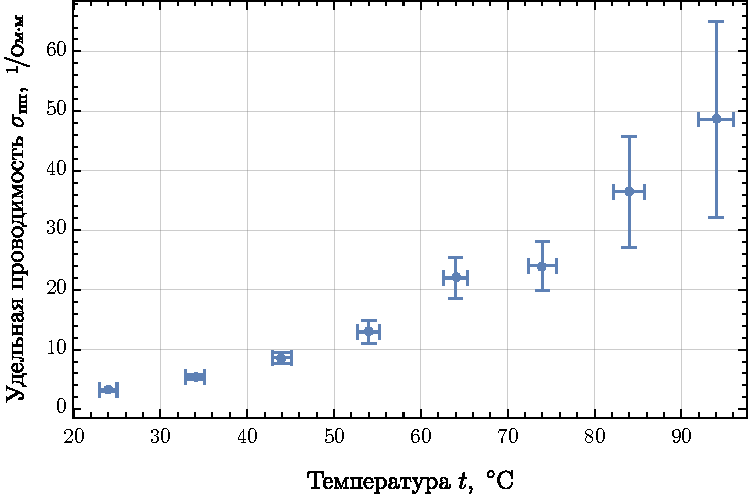
\includegraphics[width=0.8\textwidth]{3}
	\caption{График зависимости $\sigma(T)$ полупроводника}
	\label{fig:1}
\end{figure}
\begin{figure}[htpb]
	\centering
	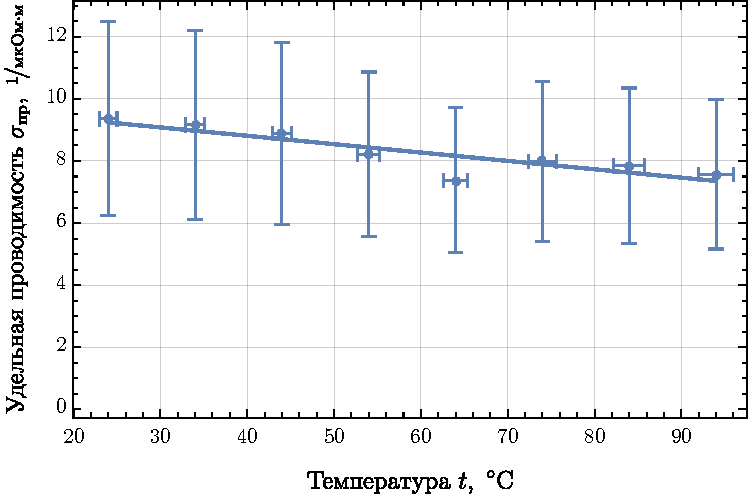
\includegraphics[width=0.8\textwidth]{2}
	\caption{График зависимости $\sigma(T)$ проводника}
	\label{fig:2}
\end{figure}
\begin{figure}[htpb]
	\centering
	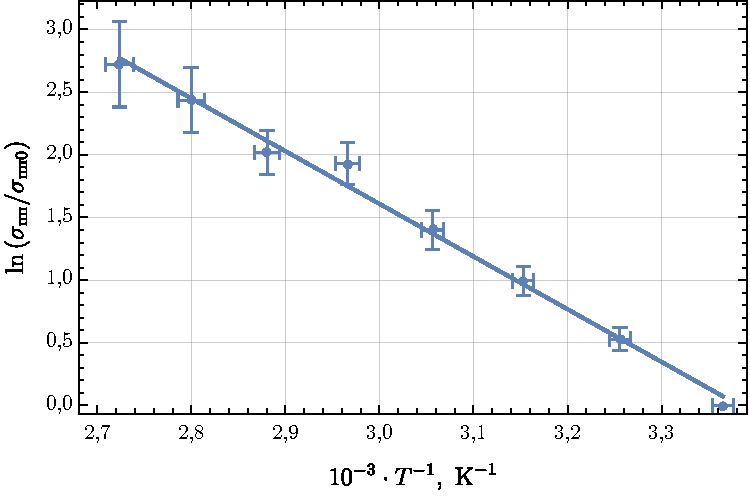
\includegraphics[width=0.8\textwidth]{1}
	\caption{График $\ln \sigma =f(1 /T)$ полупроводника}
	\label{fig:3}
\end{figure}
Для проводника (в нашем случае --- меди) коэффициент наклона графика 
\[
\frac{d\sigma}{dT}=-0,027\pm 0,006\ \frac{1}{\text{мкОм}\cdot \text{м}
\cdot \text{К}}
.\] 
Среднее значение $\sigma$ по исследуемому интервалу будет равно
\[\overline{\sigma}=8,3\pm 1,0\, \frac{1}{\text{мкОм}\cdot \text{м}}.\]
А температурный коэффициент сопротивления соответственно
\[
\alpha=- \frac{1}{\overline{\sigma}} \frac{d\sigma}{dT}=
0,0033\pm 0,0008 \, ^\circ \text{С} ^{-1}
 ,\] 
что в пределах погрешности совпадает с табличным значением
\[
\alpha_\text{Cu}\approx 0,004 \, ^\circ \text{С} ^{-1}
.\] 
По графику на рис.~\ref{fig:3} определяем коэффициент наклона
\[
	\eta=(-4,20\pm 0,15)\, \text{К}
.\] 
Откуда ширина запрещённой зоны полупроводника
\[
\Delta= -2k \eta =0,73\pm 0,03\, \text{эВ}
,\] 
что сопвадает с табличной величиной запрещённой зоны для германия
\[
\Delta_\text{Ge}\approx 0,7\,\text{эВ}
.\] 
\end{document}
